\documentclass[border=10pt]{standalone}
\usepackage[svgnames]{xcolor}
\usepackage{amsmath}
\usepackage{pgfplots}
\pgfplotsset{compat=newest}
\usepackage[sfdefault]{FiraSans}
\usepackage{FiraMono}
\renewcommand*\familydefault{\sfdefault}
\begin{document}
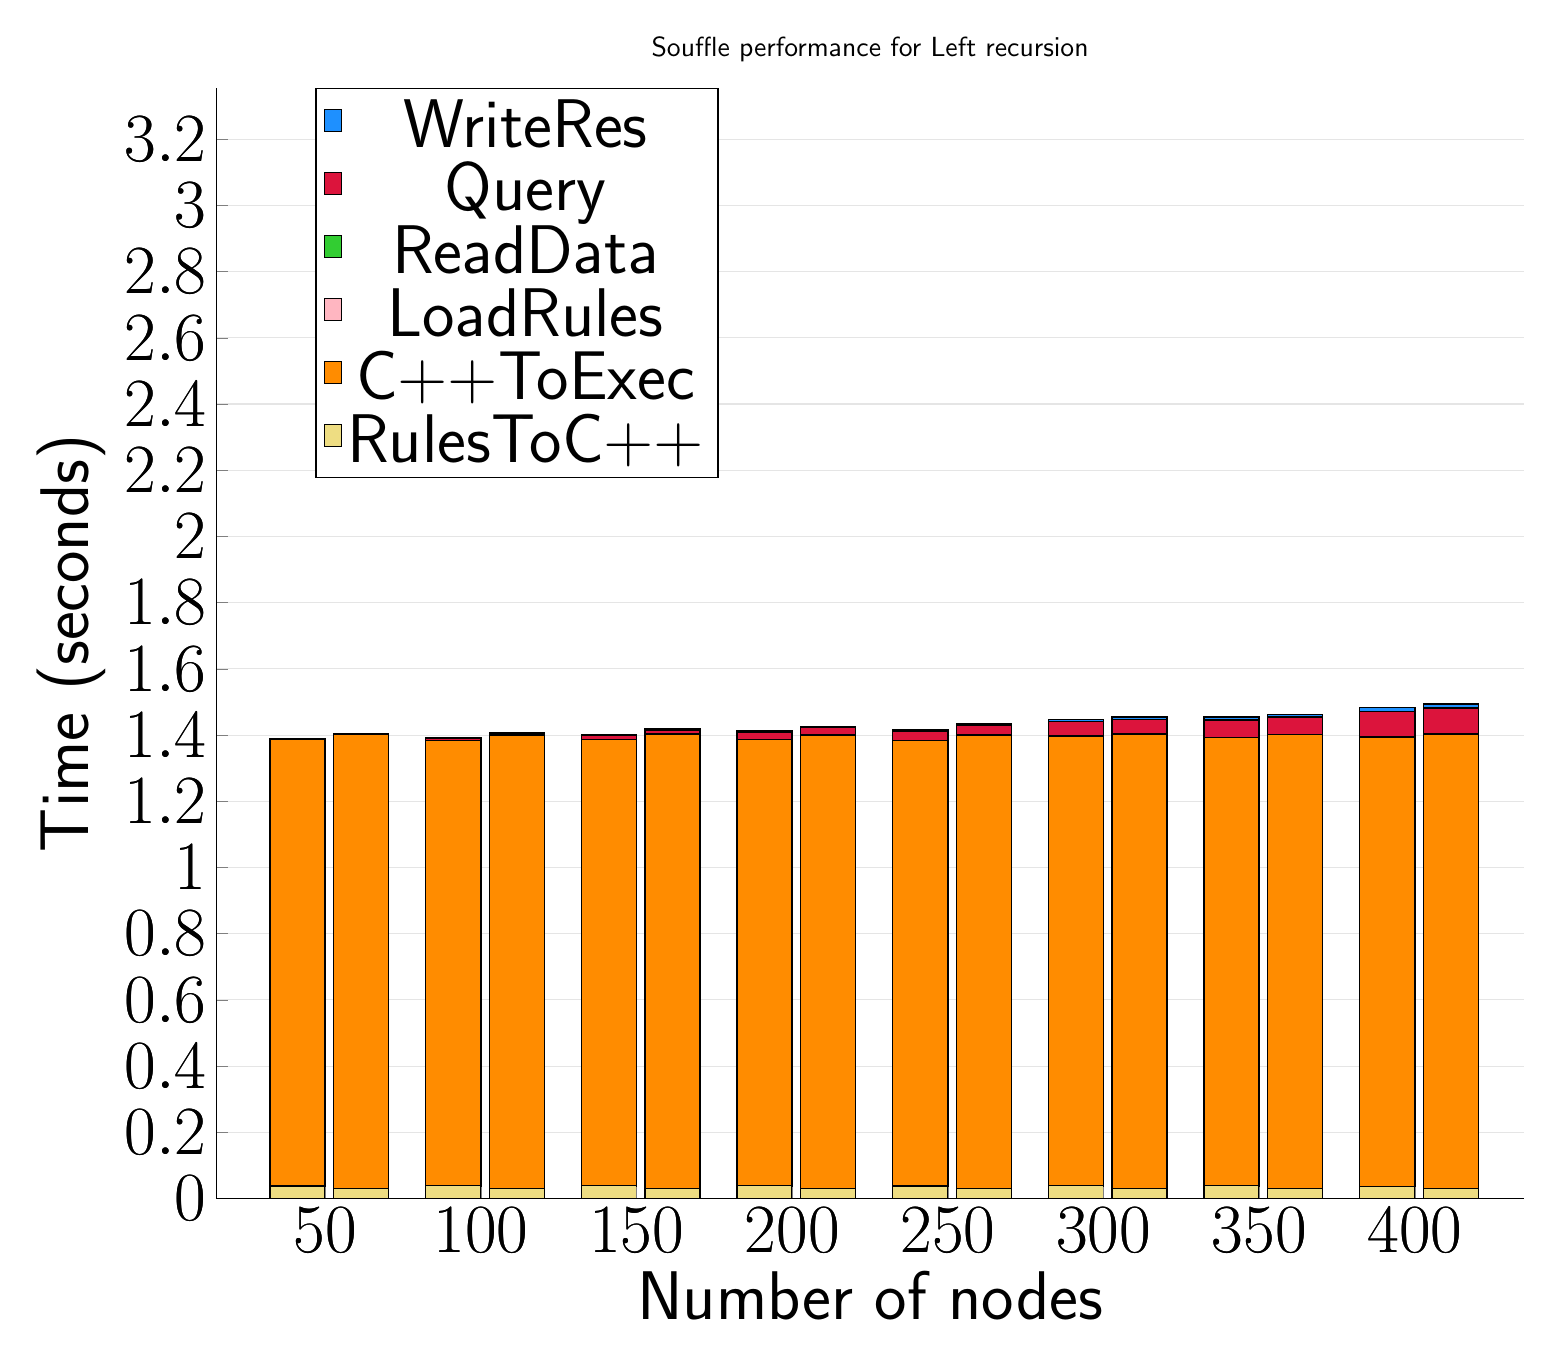
\begin{tikzpicture}
\begin{axis}[
   ybar stacked,
   title={Souffle performance for Left recursion},
   bar shift=-10pt,
   width=1.5\textwidth,
   bar width=0.7cm,
   ymajorgrids, tick align=inside,
   major grid style={draw=gray!20},
   xtick=data,
   ymin=0, ymax=3.3549999952316285,
   axis x line*=bottom,
   axis y line*=left,
   enlarge x limits=0.1,
   legend style={
       at={(0.23, 1)},
       anchor=north,
       legend columns=1,
       font=\Huge,
   },
   ylabel={Time (seconds)},
   xlabel={Number of nodes},
   label style={font=\Huge},
   tick label style={font=\Huge},
]
\addlegendimage{fill=DodgerBlue, draw=black, line width=0.2pt}
\addlegendentry{WriteRes}
\addlegendimage{fill=Crimson, draw=black, line width=0.2pt}
\addlegendentry{Query}
\addlegendimage{fill=LimeGreen, draw=black, line width=0.2pt}
\addlegendentry{ReadData}
\addlegendimage{fill=LightPink, draw=black, line width=0.2pt}
\addlegendentry{LoadRules}
\addlegendimage{fill=DarkOrange, draw=black, line width=0.2pt}
\addlegendentry{C++ToExec}
\addlegendimage{fill=LightGoldenrod, draw=black, line width=0.2pt}
\addlegendentry{RulesToC++}
\addplot +[fill=LightGoldenrod, draw=black, line width=0.5pt] coordinates {
    (50, 0.03799998760223389)
    (100, 0.03900001049041748)
    (150, 0.04000000953674317)
    (200, 0.04000000953674317)
    (250, 0.03799998760223389)
    (300, 0.039999961853027344)
    (350, 0.03899998664855957)
    (400, 0.036999964714050294)
};
\addplot +[fill=DarkOrange, draw=black, line width=0.5pt] coordinates {
    (50, 1.3480000019073486)
    (100, 1.3440000057220458)
    (150, 1.3460000038146973)
    (200, 1.3459999799728393)
    (250, 1.3449999809265136)
    (300, 1.35600004196167)
    (350, 1.352999997138977)
    (400, 1.3550000190734863)
};
\addplot +[fill=LightPink, draw=black, line width=0.5pt] coordinates {
    (50, 0.00011616670000000001)
    (100, 0.00011694170000000001)
    (150, 9.975420000000001e-05)
    (200, 0.00010002510000000001)
    (250, 0.00011344170000000002)
    (300, 0.00011345820000000001)
    (350, 0.00010943739999999999)
    (400, 9.26292e-05)
};
\addplot +[fill=LimeGreen, draw=black, line width=0.5pt] coordinates {
    (50, 0.00040764170000000006)
    (100, 0.0006016044000000001)
    (150, 0.0007363916)
    (200, 0.0009613587000000002)
    (250, 0.0010637033000000001)
    (300, 0.001374561)
    (350, 0.001415604)
    (400, 0.0017668839999999998)
};
\addplot +[fill=Crimson, draw=black, line width=0.5pt] coordinates {
    (50, 0.001235855)
    (100, 0.005648775)
    (150, 0.011505030000000001)
    (200, 0.0213866)
    (250, 0.02764119)
    (300, 0.04315207)
    (350, 0.05206255)
    (400, 0.07728429)
};
\addplot +[fill=DodgerBlue, draw=black, line width=0.5pt] coordinates {
    (50, 0.0008183375999999999)
    (100, 0.001535175)
    (150, 0.002924388)
    (200, 0.004244913)
    (250, 0.0051776209999999994)
    (300, 0.007359699)
    (350, 0.008613503)
    (400, 0.012594)
};
\end{axis}
\begin{axis}[
   ybar stacked,
   bar shift=13pt,
   width=1.5\textwidth,
   bar width=0.7cm,
   ymajorgrids, tick align=inside,
   major grid style={draw=none},
   xtick=data,
   ymin=0, ymax=3.3549999952316285,
   axis x line*=none,
   axis y line*=none,
   enlarge x limits=0.1,
   label style={font=\Huge},
   tick label style={font=\Huge},
]
\addplot +[fill=LightGoldenrod, draw=black, line width=0.5pt] coordinates {
    (50, 0.030000000000000006)
    (100, 0.030000000000000006)
    (150, 0.030000000000000006)
    (200, 0.030000000000000006)
    (250, 0.030000000000000006)
    (300, 0.030000000000000006)
    (350, 0.030000000000000006)
    (400, 0.030000000000000006)
};
\addplot +[fill=DarkOrange, draw=black, line width=0.5pt] coordinates {
    (50, 1.3730000000000002)
    (100, 1.3700000000000003)
    (150, 1.3730000000000004)
    (200, 1.3700000000000003)
    (250, 1.3700000000000003)
    (300, 1.3730000000000004)
    (350, 1.371)
    (400, 1.373)
};
\addplot +[fill=LightPink, draw=black, line width=0.5pt] coordinates {
    (50, 0.0001155)
    (100, 0.0001163)
    (150, 9.919999999999999e-05)
    (200, 9.95e-05)
    (250, 0.00011270000000000002)
    (300, 0.00011279999999999999)
    (350, 0.00010870000000000001)
    (400, 9.2e-05)
};
\addplot +[fill=LimeGreen, draw=black, line width=0.5pt] coordinates {
    (50, 0.0004068)
    (100, 0.0006006)
    (150, 0.0007356999999999999)
    (200, 0.000959)
    (250, 0.0010628999999999999)
    (300, 0.0013739000000000002)
    (350, 0.0014149)
    (400, 0.0017656999999999998)
};
\addplot +[fill=Crimson, draw=black, line width=0.5pt] coordinates {
    (50, 0.0012343)
    (100, 0.005648200000000001)
    (150, 0.0114977)
    (200, 0.0213543)
    (250, 0.027607100000000002)
    (300, 0.0431208)
    (350, 0.051973300000000014)
    (400, 0.0771452)
};
\addplot +[fill=DodgerBlue, draw=black, line width=0.5pt] coordinates {
    (50, 0.0005489000000000001)
    (100, 0.0015336)
    (150, 0.0027530999999999996)
    (200, 0.0042326)
    (250, 0.005171)
    (300, 0.0073131)
    (350, 0.0086033)
    (400, 0.012383700000000001)
};
\end{axis}
\end{tikzpicture}

\end{document}
